\documentclass[UTF-8]{ctexbeamer}
\usepackage{amsmath,animate,bm,amssymb,hyperref,graphicx,mathrsfs}
\usepackage{hyperref}


\usetheme{Darmstadt} 
\usecolortheme{dolphin} 
\title{数据及其描述:统计量}
%\subtitle{I.7 I.8 existence theory}
\author{董浚哲}
\date{\today}

\begin{document}
\newcommand{\wrt}{w.r.t.}
\newcommand{\dd}{\,\mathrm{d}}
\newcommand{\st}{\text{ s.t. }}
\newcommand{\pp}[2]{\frac{\partial #1}{\partial #2}}
\newcommand{\dif}[2]{\frac{\mathrm{d} #1}{\mathrm{d} #2}}


\newtheorem{Thm}{定理}[section]
%\newtheorem{Lemma}[Thm]{引理}
\newtheorem{Prop}[Thm]{命题}
\newtheorem{Cor}[Thm]{推论}
\newtheorem{Def}{定义}[section]
\newtheorem{Rmk}{注}[section]
\newtheorem{Eg}{例}[section]
%\newenvironment{solution}{\begin{proof}[Solution]}{\end{proof}}

\begin{frame}
\titlepage
\end{frame}

\section{数据和变量}
\begin{frame}
所有数据构成集合 $\Omega$ 。概率$P$ 是概率空间 $(\Omega,\mathscr{A}$ )上的测度,且使得 $P(\Omega)=1$ ,其中 $\Omega$ 是数据集。

$ (\Omega,\mathscr{A},P) $ 上的可测函数称为(随机)变量。

(从数据库存储信息的角度看)依 $\Omega$ 的不同,随机变量可能被分为:
\begin{itemize}
\item 定量变量
  \begin{itemize}
  \item 连续型变量
  \item 离散型变量
  \end{itemize}
\item 定性变量
\end{itemize}
若$\Omega$上有序关系,则称为定序变量。
\end{frame}

\begin{frame}
  随机变量$X$是概率空间上的可测函数。对其可以定义矩统计量:$\nu_{k}=E(X^{k})$:$k$阶原点矩,$\mu_{k}=E((X-E(X)^{k}))$:k阶中心矩。特别地:
  \begin{itemize}
    
  \item 方差:$\sigma^{2}=Var(X)=\mu_{2}$
  \item 偏度:$\beta_{s}=Skew(X)=\frac{\mu_{3}}{\mu_{2}^{\frac 3 2}}$
  \item 峰度:$\beta_{k}=Kurt(X)=\frac{\mu_{4}}{\mu_{2}^{2}}$
  \end{itemize}
\end{frame}

\begin{frame}
  \begin{Lemma}
    设$a\neq 0$,随机变量$X,Y$的密度函数分别为$p_{X}(x),p_{Y}(y)$,且其联合分布为$f(x,y)$,则
    $Z=X+Y$的密度函数为$p(z)=\int_{-\infty}^{\infty}f(x,z-x)\dd x$。特别地,当$X,Y$独立时,$p(z)=\int_{-\infty}^{\infty}f_{X}(x)f_{Y}(z-x)\dd x$
      \end{Lemma}
      % 
\includegraphics[scale=0.3]{proof_of_sum.png}
      
  \begin{proof}
  记$D_{z}=\{(x,y)|x+y\leq z\}$,则
  \begin{align*}
    F_{Z}(z)&=P(Z\leq z)=P(X+Y\leq z)\\
            &=\iint_{D_{z}}f(x,y)\dd x\dd y=\int_{-\infty}^{\infty}(\int_{-\infty}^{z-x}f(x,y))\dd x\\
    f_{Z}(z)=&\dif{}{z}F_{Z}(z)=\int_{-\infty}^{\infty}f(x,z-x)\dd x
  \end{align*}
  \end{proof}
\end{frame}


\begin{frame}
  \begin{Lemma}[随机变量之商的密度函数]
    设$X,Y$是具有密度函数$f_{X}(x),f_{Y}(y)$的随机变量,则$Z=\frac{Y}{X}$的密度函数为
    \[f_{Z}(z)=\int_{-\infty}^{\infty}|x|f_{Y}(xz)f_{X}(x)\dd x\]
  \end{Lemma}
    $$
F_{Z}(z)=P\left(\frac{Y}{X} \leq z\right)=P(Y \geq z X, X<0)+P(Y \leq z X, X>0)
$$
$$
=\int_{-\infty}^{0}\left(\int_{z x}^{+\infty} f_{Y}(y) \mathrm{d} y\right) f_{X}(x) \mathrm{d} x+\int_{0}^{\infty}\left(\int_{-\infty}^{z x} f_{Y}(y) \mathrm{d} y\right) f_{X}(x) \mathrm{d} x
$$
再取微分得:
$$
\begin{aligned}
f_{Z}(z)=\frac{\mathrm{d} F_{Z}(z)}{\mathrm{d} z} &=\int_{-\infty}^{0}\left(-x f_{Y}(x z)\right) f_{X}(x) \mathrm{d} x+\int_{0}^{+\infty}\left(x f_{Y}(x z)\right) f_{X}(x) \mathrm{d} x \\
&=\int_{-\infty}^{+\infty}|x| f_{Y}(x z) f_{X}(x) \mathrm{d} x
\end{aligned}
$$
\end{frame}

\begin{frame}
  \begin{Thm}
    设$X$为连续随机变量,密度函数为$f(x)$。设$U=\phi(X)$,其中$X=\phi^{-1}(U)=\psi(U)$。设$U$的密度函数为$g(u)$,则
    \[g(u)=f(x)\left|\dif{x}{u}\right|=f(\psi(u))|\psi'(u)|\]
  \end{Thm}
  \begin{proof}
    对$\phi$单调递增的情况进行证明,单调递减的情况是类似的。考察$U$的分布函数$F_{U}(u)$:
    \[F_{U}(u)=P(U\leq u)=P(\phi(X)\leq U)=P(X\leq \psi(u))=F_{X}(\psi(u))\]
    再取微分即得。
  \end{proof}
  $X\sim p(x)\Rightarrow aX\sim \frac{1}{|a|}p(\frac{1}{a}x)$
\end{frame}

\begin{frame}
  Gamma函数:$\Gamma(x)=\int_{0}^{\infty}t^{x-1}e^{-t}\dd t$

  $\Gamma(x+1)=x\Gamma(x),\Gamma(\frac{1}{2})=\sqrt{\pi}$

  Beta函数:$B(p,q)=\int_{0}^{1}x^{p-1}(1-x)^{q-1}\dd x=\int_{0}^{\infty}\frac{x^{p-1}}{(1+x)^{p+q}}\dd x$

  $B(p,q)=\dfrac{\Gamma(p)\Gamma(q)}{\Gamma(p+q)}$
\end{frame}
\section{总体、样本、统计量}

\subsection{总体}
\begin{frame}
  我们把研究对象的全体称为\textbf{总体},其中每个成员称为\textbf{个体}。我们用随机变量及其分布刻画总体的性质。

(故“从某总体中抽样”与“从某分布中抽样”同义。)

多个随机变量取直积得一随机向量,其分布称为\textbf{联合分布}。常假设随机变量之间有关联,故常假定一些“条件分布”的形式。
\begin{Eg}
在文本数据分析中,个体是一篇篇文章。每篇文章可以对应成一个 $P_1$ 维向量。表示该文章在$P_1$个词语上的词频。我们认为这个$ P_1$维向量服从一定的概率分布。
\end{Eg}
\begin{Eg}
  E.g. 在图像分析中,个体是一张张图片,对应的数量指标是$ P_2$维向量,表示图片在$ P_2$个像素点的像素值,服从一个$ P_2$维的概率分布。
  \end{Eg}
\end{frame}

\subsection{样本}

\begin{frame}
  不同于普查,抽样只从总体抽取若干个体进行检查或观察,用所获得的数据对总体进行统计推断。
  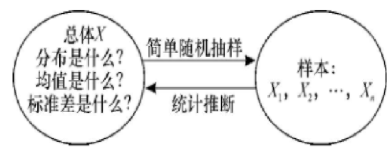
\includegraphics{sample.png}
\end{frame}

\begin{frame}
抽样所抽出部分个体之集合称\textbf{样本},其元素称\textbf{样品},样品个数称\textbf{样本(容)量}。容量为 $n$ 的样本可视为$n$维随机向量,以大写字母$X_1,\cdots,X_n$表示,而其观测值则以$x_1,\cdots,x_n$表示。$\mathscr{A}$,即一切可能的观测值之全体,称为 $n$ 维样本空间。

作为理想的抽样方法,简单随机抽样得到的样品是独立同分布(iid)的,称\textbf{简单随机样本}或\textbf{独立同分布样本}。
\end{frame}

\subsection{统计量}
\begin{frame}
  \begin{Def}
  不含任何未知参数的样本函数称为统计量。
  
  \end{Def}

常见的统计量有:
\begin{itemize}
\item 样本均值:$\bar X=\dfrac{1}{n}\sum\limits_{i=1}^n X_i$
\item  样本方差:$S^2=\dfrac{1}{n-1}\sum\limits_{i=1}^n (X_i-\bar X)^2$
\item  样本标准差:$S=\sqrt{S^2}$
\end{itemize}
\end{frame}

\begin{frame}
  $\bar X$是总体期望$\mu$的估计。由于$E(\bar X)=\mu$,故曰用样本均值估计总体期望时*没有系统偏差*。

  由于 $\sum^n_{i=1}(X_i-\bar X)=0$,$n$ 个独立偏差只有 $n-1$ 个自由度。
  为累计各偏差,采用偏差平方和 $Q=\sum\limits_{i=1}^n (X_i-\bar X)^2$ 度量数据的散布大小。

又为消除样本量之影响,用平均偏差平方和 $S_n^2=\frac{Q}{n}$度量数据的散布大小。因$E(S_n^2)=(1-\frac{1}{n})\sigma^2$,$S_n^2$是对总体方差 $\sigma^2$ 的估计,故称\textbf{未修正的样本方差}。

修正系数得到样本方差$S^2$,$E(S^2)=\sigma^2$,是总体方差$\sigma^2$的估计

$S$ 的单位与数据相同便于解释与运算(这使得 $\mu$的区间估计$\bar X\pm kS$ 是有意义的)。它是标准差 $\sigma$ 的估计,用于度量样本散布的大小。
\end{frame}

\section{从样本认识总体的图表方法}

\subsection{直方图}

\begin{frame}
  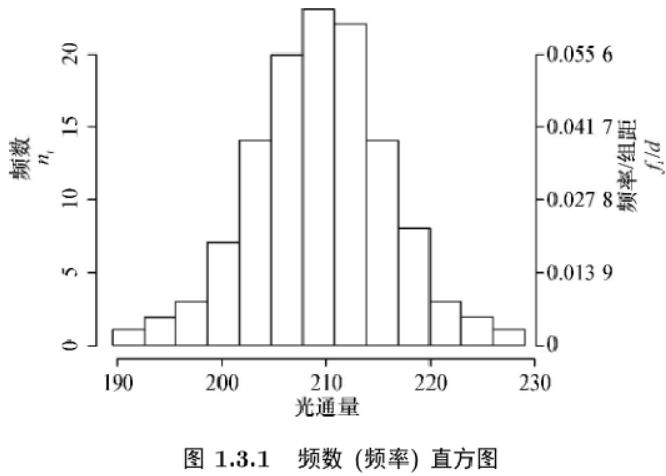
\includegraphics[scale=0.5]{rate.png}

可以绘制频率(频数)直方图来反映总体密度函数的形状。上述直方图是无偏的,但有时直方图显示数据是有偏的。
\end{frame}

\begin{frame}
  \begin{Def}
    偏度(skewness)是描述统计量偏离对称程度的统计量。
    \begin{itemize}
    \item $Skew(X)<0$,称负偏态或\textbf{左偏},平均值<中位数。
    \item $Skew(X)>0$,称正偏态或$\textbf{右偏}$,平均值>中位数。
    \end{itemize}
  \end{Def}
\end{frame}




\subsection{经验分布函数}
\begin{frame}
  设总体$X$的概率密度函数为$f(x)$,累计分布函数为$F(x)$。

把n个观测值$X_1,X_2,\cdots,X_n$视为某离散随机变量等可能取的值(即$P(X_k)=\frac{1}{n}\quad\forall 1\leq k\leq n$)。将观测值升序重新编号为$x_{(1)},\cdots,x_{(n)}$得到该样本的\textbf{经验分布函数}:

$$
F_n(x)=\begin{cases}
0& x<x_{(1)}\\ 
\frac{k}{n}& x_{(k)}<x<x_{(k+1)}\quad \forall 1\leq k<n\\
1&x>x_{(n)}
\end{cases}
$$
\end{frame}

\begin{frame}
  \begin{Thm}[Glivenko-Cantelli]
    设总体的累计分布函数为$F(x)$,$\forall n\in\mathbb{N}$,$F_n(x)$是关于从该总体中抽取的样本$x_1,\cdots,x_n$的经验分布函数,则
\[P(\lim\limits_{n\to\infty}\{x\in \Omega|F_n(x)\neq F(x)\})=0\]
\end{Thm}


\includegraphics[scale=0.3]{Glivenko-Cantelli.png}
\end{frame}

\begin{frame}
  经验分布函数的各阶矩称为\textbf{样本矩}或\textbf{矩统计量}(moment)。特别地
\begin{itemize}
\item$A_k=\frac{1}{n}\sum_{i=1}^nX_i^k$ 称样本k阶(原点)矩
  
\item$B_k=\frac{1}{n}\sum_{i=1}^n( X_i-\bar X)^k$ 称样本k阶中心矩
\end{itemize}

可以用它们构造诸如样本偏度($\hat\beta_s=B_3/B_2^{\frac 3 2}$)、样本峰度($\hat b_k=B_4/B_2^2-3$)等统计量。
\end{frame}

\subsection{高维数据的图表展示方法}
%To be continued

\subsection{数据变换}
%To be continued

\section{次序统计量}
\begin{frame}
  \begin{Def}
    设$X_1,\cdots, X_n$ 是取自总体$X$的$n$个样本。称$X_{(k)}$为该样本的第$k$个次序统计量。假如每当获得样本观测值后将其从小到大排序可得如下有序样本:

$$
x_{(1)}\leq x_{(2)}\leq\cdots\leq x_{(n)}
$$

其中$x_{(k)}$是$X_{(k)}$的取值。特别地,$X_{(1)},X_{(n)}$分别称该样本的最小、最大统计量。
  \end{Def}
\end{frame}

\begin{frame}
  \begin{Eg}
    $X$的分布为取0,1,2的离散均匀分布。今抽取容量为3的样本,得到次序统计量的分布与联合分布如下
    % 先展示总结果
    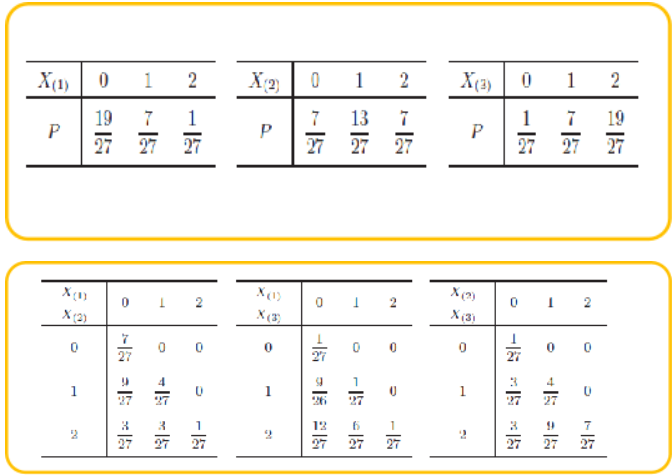
\includegraphics[scale=0.4]{joint.png}
    
    可见$(X_1,X_2,X_3)$与$(X_{(1)},X_{(2)},X_{(3)})$ 不同,且任意两个次序统计量的联合分布也是不同的。任意两个次序统计量是不独立的。
  \end{Eg}
  
\end{frame}

\subsection{样本极差}
\begin{frame}
  $R=x_{(n)}-x_{(1)}$ 称为样本极差。这是方差的反映。

  事实上,令$g(x_i,x_j)=\frac{1}{2}(x_i-x_j)^2$,则$E[g(x_i,x_j)]=\sigma^2$,即:这是方差的无偏估计。将这$C_n^2$个估计取平均值就得到样本方差$S^2$

  
\includegraphics[scale=0.3]{proof_of_average.png}
\end{frame}

\subsection{p分位数}
\begin{frame}
  对给定的$p\in(0,1)$,称

$$
m_d=
\begin{cases}
\frac{1}{2}[x_{[np]}+x_{[np]+1}] &np\not\in \mathbb{Z}\\
x_{([np]+1)}& np\in \mathbb{Z}
\end{cases}
$$

为该样本的p分位数。特别地,$p=\frac{1}{2}$时,$m_d$为中位数。

p分位数是对$F(x_p)=p$ 的解的估计。
\end{frame}

\subsection{箱线图与QQ图}

\begin{frame}
  取下列五个次序统计量作“五数概括”
\[x_{(1)},Q_1,m_d,Q_3,x_{ (n)}\]
(其中$ Q_1=m_{0.25}$和$ Q_3=m_{0.75}$分别称为样本的第一和第三四分位数, $ m_d$为中位数。)
由此得到的图形称为箱线图,该图由一个箱子和两个线段连接而成:

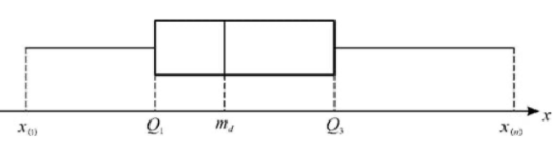
\includegraphics[scale=0.9]{box.png}
\end{frame}
\begin{frame}
  箱线图可用来对总体的分布形状进行大致的判断。特别地,用于区分左偏分布、对称分布和右偏分布。
  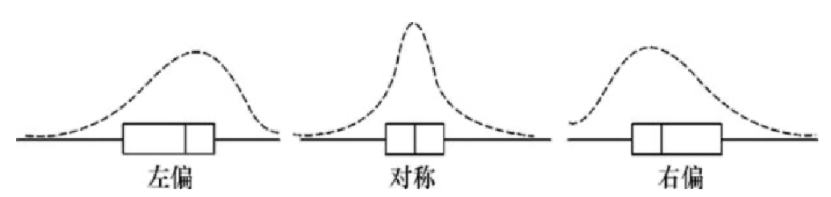
\includegraphics[scale=0.5]{lmr.png}
\end{frame}

\begin{frame}
  QQ图(quantile-quantile plot):分位数-分位数图,取两个样本(或样本与标准分布)的各分位数作散点图,用于检验两组样本是否来自同一分布,或样本是否来自给定分布。

  若两者分布一致,则图像落在直线$y=x$上;若两者呈线性相关,则图像落在直线上(不一定是$y=x$)

  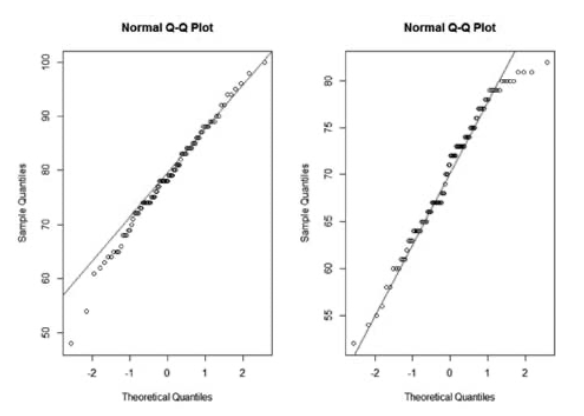
\includegraphics[scale=0.3]{QQ_plot.png}
\end{frame}

\section{抽样分布}

\subsection{样本均值的抽样分布}
\begin{frame}
  \begin{Def}
    统计量的概率分布称为\textbf{抽样分布}。
  \end{Def}
  若总体分布为$N(\mu,\sigma^2)$,则$\bar X$的精确分布为$N(\mu,\frac{\sigma^2}{n})$

  若总体分布未知或不是正态分布但$\mu,\sigma^2$存在,则由中心极限定理,$\bar X\sim N(\mu,\frac{\sigma^2}{n})$

  \begin{Thm}[Kolmogorov 大数定律(强)]
    设$\{X_{n}\}$是独立同分布的随机变量列,且$\mu=E(X_{n})<+\infty$,则
    \[\lim\limits_{n\to\infty}\frac{\sum_{i=1}^{n} X_{i}}{n}=\mu\quad a.e.\]
  \end{Thm}
\end{frame}

\subsection{正态总体各统计量的分布}
\begin{frame}
  \begin{Def}
  设$u_1,\cdots,u_m$ 为$m$个iid的标准正态变量,则$Y=\sum_{i=1}^m u_i^2$ 的分布称为自由度$m$的$\chi^2$分布,记作$\chi^2(m)$,其密度函数为:
\[p(y)=\frac{1}{\Gamma(\frac{m}{2})}2^{-\frac{m}{2}}y^{\frac{m}{2}-1}e^{-\frac{y}{2}}\]
\end{Def}
\begin{Thm}
  设$X=(X_1,\cdots,X_n)$为来自正态总体$N(\mu,\sigma^2)$的样本,$\bar X,S^2$分别为其样本均值和样本方差,则
\begin{itemize}
\item $\bar X\sim N(\mu,\frac{\sigma^2}{n})$
  
\item $\frac{n-1}{\sigma^2}S^2\sim\chi^2(n-1)$
  
\item $\bar X$与$S^2$相互独立
\end{itemize}

\end{Thm}
\end{frame}

\begin{frame}
  \begin{Lemma}
    设两个随机向量$X=(X_1,\cdots,X_n)',Y=(Y_1,\cdots,Y_n)'$,且有方阵$A=(a_{ij})_{n\times n}$使得$Y=AX$,则$E(Y)=AE(X)$,$Var(Y)=AVar(X)A'$
  \end{Lemma}

\begin{proof}[引理的证明]
  $Y=AX\Rightarrow Y_{i}=\sum_{j=1}^{n}a_{ij}X_{j}\Rightarrow E(Y_{i})=\sum_{j=1}^{n}a_{ij}E(X_{j})\Rightarrow E(Y)=AE(X)$
%\end{proof}

%\end{frame}

%\begin{frame}
%\begin{proof}[引理的证明(续)]
  \[\begin{aligned}
Var(Y)&=E[(Y − E(Y))(Y − E(Y))']\\
&=E[(AX − AE(X))(AX −AE(X))']\\
&=AE[(X − E(X))(X − E(X))']A'=AVar(X)A'
\end{aligned}\]
\end{proof}
\end{frame}

\begin{frame}
  \begin{proof}[定理的证明]
    记$X=(X_{1},\cdots,X_{n})'$,则$E(X)=(\mu,\cdots,\mu)'$,$Var(X)=\sigma^{2} I$

    取$A$为正交矩阵,使得$a_{ik}\equiv \frac{1}{\sqrt{n}}\quad \forall 1\leq k\leq n$。
    (这就要求$\sum\limits_{k=1}^{n}a_{mk}\equiv 0\quad \forall 2\leq m\leq n$)
    取$Y=AX$,则由正态分布之线性性知$Y$尤为正态分布,且
    \[E(Y)=AE(X)=(\sqrt{n}\mu,0,\cdots,0)',Var(Y)=\sigma^{2}I\]
    % 计算过程……?
    故$Y_{1}\sim N(\sqrt{n}\mu,\sigma^{2}),Y_{k}\sim N(0,\sigma^{2})\quad 2\leq k\leq n$且相互独立。

    注意到$\bar X=\frac{1}{\sqrt{n}}Y_{1}$,故$\bar X\sim N(\mu,\frac{\sigma^{2}}{n})$。
\end{proof}
  \end{frame}
  
\begin{frame}
    \begin{proof}[定理的证明(续)]
    又注意到$\sum_{i=1}^{n}Y_{i}^{2}=Y'Y=X'A'AX=X'X=\sum_{i=1}^{n}X_{i}^{2}$,故
    \[(n-1)S^{2}=\sum_{i=1}^{n}(X_{i}-\bar X)^{2}=\sum_{i=1}^{n}X_{i}^{2}-(\sqrt n \bar X)^{2}=\sum_{i=1}^{n}Y_{i}^{2}-Y_{1}^{2}=\sum_{i=2}^{n}Y_{i}^{2}\]
    故$\frac{n-1}{\sigma^{2}}S^{2}=\sum_{i=2}^{n}(\frac{Y_{i}}{\sigma})^{2}\sim \chi^{2}(n-1)$

    再注意到$\bar X$只与$Y_{1}$有关,$S^{2}$只与$Y_{2},\cdots,Y_{n}$有关,故二者独立。
  \end{proof}
\end{frame}

\begin{frame}
  \begin{Def}
    若随机变量$t$的密度函数为
    \[p(t;n)=\frac{\Gamma(\frac{n+1}{2})}{\sqrt{n\pi}\Gamma(\frac{n}{2})}(1+\frac{t^{2}}{n})^{-\frac{n+1}{2}}=\frac{1}{\sqrt{n}}B(\frac{1}{2},\frac{n}{2})^{-1}(1+\frac{t^{2}}{n})^{-\frac{n+1}{2}}\quad t\in\mathbb{R}\]
    则称$t$服从自由度为$n$的(标准)$t$分布,记做$t\sim t(n)$。
  \end{Def}
  一般的以$(\mu,\sigma^{2},n)$为数学期望、方差、自由度的$t$分布的密度函数为:
  \[p(x)=\frac{1}{\sqrt{n}\sigma}B(\frac{1}{2},\frac{n}{2})^{-1}(1+\frac{(x-\mu)^{2}}{n\sigma^{2}})^{-\frac{n+1}{2}}\]
\end{frame}

\begin{frame}
  \begin{Thm}
    设$X\sim N(0,1),Y\sim \chi^{2}(n)$且独立,则$t=\frac{X}{\sqrt{Y/N}}\sim t(n)$
  \end{Thm}
  \begin{proof}
    首先考察$Z=\sqrt{\frac{Y}{N}}$的密度函数$f_{z}(z)$。因$Z>0$,故$f_{z}(z)\equiv 0\quad \forall z\leq 0$。又$F_{Z}(z)=P(Z\leq z)=P(\sqrt{\frac{Y}{N}}\leq z)=P(Y\leq nz^{2})=F_{Y}(nz^{2})$,故
    \[f_{Z}(z)=\dif{}{z}F_{Y}(nz^{2})=\Gamma(\frac{n}{2})^{-1}2^{-\frac n 2+1}n^{\frac n 2}z^{n-1}e^{-\frac{nz^{2}}{2}}\quad \forall z>0\]
  \end{proof}
\end{frame}

\begin{frame}
  \begin{proof}[证明(续)]
    应用随机变量的商的密度函数的公式得到:
    \begin{equation}
\begin{aligned}
P_{T}(t ; n) &=\int_{-\infty}^{\infty}|z| f_{z}(z) f_{x}(z t) \dd z \\
&=\int_{0}^{\infty} z \frac{1}{\sqrt{2 \pi}} e^{-\frac{z^{2} t^{2}}{2}} \frac{1}{2^{\frac{n}{2}-1} \Gamma\left(\frac{n}{2}\right)} n^{\frac{n}{2}} z^{n-1} e^{-\frac{n z^{2}}{2}} \dd z \\
&=\frac{n ^{\frac{n}{2}}}{\sqrt{\pi} 2^{\frac{n-1}{2}} \Gamma\left(\frac{n}{2}\right)} \int_{0}^{\infty} z^{n} e^{-\frac{z^{2}}{2}\left(n+t^{2}\right)} \dd z \quad \text{令}u=\frac{n+t^{2}}{2}z^{2}\\
& \frac{1}{\sqrt{n \pi} \Gamma\left(\frac{n}{2}\right)\left(1+\frac{t^{2}}{n}\right)^{\frac{n+1}{2}}} \int_{0}^{\infty} u^{ \frac{n+1}{2}}e^{-u} \dd u \\
&=\frac{\Gamma\left(\frac{n+1}{2}\right)}{\sqrt{n \pi} \Gamma\left(\frac{n}{2}\right)}\left(1+\frac{t^{2}}{n}\right)^{-\frac{n+1}{2}}
\end{aligned}
\end{equation}
  \end{proof}
\end{frame}


\begin{frame}
  \begin{Thm}
    设$X_{1},\cdots,X_{n}$是来自总体$N(\mu,\sigma^{2})$的样本,$\bar X,S$分别为其样本均值和样本标准差,则
    \[t=\frac{\sqrt{n}(\bar X-\mu)}{S}\sim t(n-1)\]
  \end{Thm}
  \begin{proof}
    注意到$t=\frac{\bar X-\mu}{\sigma/\sqrt{n}}/\sqrt{\frac{(n-1)S^{2}}{\sigma^{2}}/(n-1)}$。而$\frac{\bar X-\mu}{\sigma/\sqrt{n}}\sim N(0,1), \frac{(n-1)S^{2}}{\sigma^{2}}\sim \chi^{2}(n-1)$,由上述定理即得。
  \end{proof}
\end{frame}

\begin{frame}
  t分布的密度函数图像关于纵轴对称。其形状与标准正态分布的密度函数类似,只是峰比标准正态分布低一些,尾部的概率比标准正态分布大。
  \begin{Prop}
    设$X\sim t(n)$,则
    \begin{itemize}
    \item $n=1$时,$X$服从标准Cauchy分布($s=1,t=0$):
      \[f_{X}(x)=\frac{1}{s\pi(1+(\frac{x-t}{s})^{2})}\]
      该分布期望不存在。
    \item $n>1$时,$E(X)=0$;$n>2$时,$Var(X)=\frac{n}{n-2}$
      
    \item $n\to\infty$时,$t(n)$的极限分布为标准正态分布。一般在$n>30$时便可用标准正态分布进行近似。
    \end{itemize}
  \end{Prop}
\end{frame}

\begin{frame}
  显然$n>1$时,$p(x)$是偶函数,故$E(X)=0$。
\begin{align*}
  Var(X)&=E(X^{2})-[E(X)]^{2}=E(X^{2})\\
        &=\int_{-\infty}^{\infty}x^{2}p(x)\dd x=2\int_{0}^{\infty}x^{2}p(x)\dd x\\
        &=2c\int_{0}^{\infty}x^{2}(1+\frac{x^{2}}{n})^{-\frac{n+1}{2}}\dd x\quad \text{令 }t=\frac{x^{2}}{n}\\
        &=2c\int_{0}^{\infty}nt(1+t)^{-\frac{n+1}{2}}\frac{\sqrt{n}}{2}\frac{1}{\sqrt{t}}\dd t\\
        &=cn^{\frac{3}{2}}\int_{0}^{\infty}t^{\frac{3}{2}-1}(1+t)^{-\frac{3}{2}-(\frac{n}{2}-1)}\dd t\\
  &=cn^{\frac 3 2}B(\frac{3}{2},\frac{n}{2}-1)=n\frac{B(\frac{1}{2}+1,\frac{n}{2}-1)}{B(\frac{n}{2},\frac{1}{2})}=\frac{n}{n-2}
  \end{align*}
  
\end{frame}


\begin{frame}
  \begin{Lemma}[Slutski]
    设$\{X_{n}\},X,\{Y_{n}\}$是随机变量,$c\in\mathbb{R}$,且$X_{n}\to X\quad a.e.$,$Y_{n}\to c\quad \text{in measure}$,则\[X_{n}+Y_{n}\to X+c\quad a.e.\]\[X_{n}Y_{n}\to cX\quad a.e.\]
  \end{Lemma}
  
  已知$\frac{X}{\sqrt{Y/n}}\sim t(n)$,其中$X\sim N(0,1),Y\sim \chi^{2}(n)$。又$\sum_{i=1}^{n}X_{i}^{2}$,故由大数定律$\lim\limits_{n\to\infty}\frac{Y}{n}=E(X_{i}^{2})=E(X_{i}^{2})-[E(X_{i})]^{2}=Var(X_{i})=1\quad a.e.$,故由Slutski定理,$\lim\limits_{n\to\infty}t(n)=X$。
\end{frame}

\begin{frame}
  \begin{Thm}
  设$X_{1}\sim \chi^{2}(n_{1}),X_{2}\sim\chi^{2}(n_{2})$且独立,则$\dfrac{\frac{X_{1}}{n_{1}}}{\frac{X_{2}}{n_{2}}}$的概率密度函数为:
\begin{equation*}
  f(x;n_{1},n_{2})=
    \begin{cases}
      0&x\leq 0\\
      B(\frac{n_{1}}{2},\frac{n_{2}}{2})^{-1}
       % \Gamma(\frac{n_{1}+n_{2}}{2})}{\Gamma(\frac{n_{1}}{2})\Gamma(\frac{n_{2}}{2})}
        (\frac{n_{1}}{n_{2}})^{\frac{n_{1}}{2}}x^{\frac{n_{1}}{2}-1}(1+\frac{n_{1}}{n_{2}}x)^{-\frac{n_{1}+n_{2}}{2}}& x>0
    \end{cases}
  \end{equation*}
\end{Thm}
这一分布称为自由度$n_{1},n_{2}$的$F$分布。

特别地,注意到$\frac{S^{2}}{\sigma^{2}}\sim\frac{\chi^{2}(n-1)}{n-1}$,取$n_{1}=m-1,n_{2}=n-1$则得到两个正态总体的方差比的分布。
\end{frame}

\begin{frame}
  \begin{proof}
    $Z=\frac{X_{1}}{X_{2}}$的密度函数为:(其中换元$u=\frac{x_{2}}{2}(1+z)$)
$$
\begin{aligned}
p_{Z}(z) &=\int_{0}^{\infty} x_{2} p_{1}\left(z x_{2}\right) p_{2}\left(x_{2}\right) d x_{2} \\
&=\frac{z^{\frac{n_{1}}{2}-1}}{\Gamma\left(\frac{n_{1}}{2}\right) \Gamma\left(\frac{n_{2}}{2}\right) 2^{\frac{n_{1}+n_{2}}{2}}} \int_{0}^{\infty} x_{2}^{\frac{n_{1}+n_{2}}{2}-1} e^{-\frac{x_{2}}{2}(1+z)} d x_{2}\\
&=\frac{z^{\frac{n_{1}}{2}-1}(1+z)^{\frac{n_{1}+n_{2}}{2}}}{\Gamma\left(\frac{n_{1}}{2}\right) \Gamma\left(\frac{n_{2}}{2}\right)} \int_{0}^{\infty} u^{\frac{n_{1}+n_{2}}{2}-1} e^{-u} d \dd u\\
&=\frac{\Gamma\left(\frac{n_{1}+n_{2}}{2}\right)}{\Gamma\left(\frac{n_{1}}{2}\right) \Gamma\left(\frac{n_{2}}{2}\right)} z^{\frac{n_{1}}{2}-1}(1+z)^{-\frac{n_{1}+n_{2}}{2}} \quad z>0
\end{aligned}
$$
再代入$F=\frac{n_{2}}{n_{1}}Z\Rightarrow p_{F}(z)=\frac{n_{1}}{n_{2}}p_{Z}(\frac{n_{1}}{n_{2}}z)$整理即得。
\end{proof}
\end{frame}

\begin{frame}
  %Geogebra展示F分布
  \begin{Thm}
    设$X\sim F(x;n_{1},n_{2})$,则
    \begin{itemize}
    \item $n_{1}\in \{1,2\}$时,$f_{X}(x)$单调递减;否则呈右偏的单峰分布。
    \item $n_{2}>2$时,$E(X)=\frac{n_{2}}{n_{2}-2}$;$n_{2}>4$时,$Var(X)=\frac{2n_{2}^{2}(n_{1}+n_{2}-2)}{n_{1}(n_{2}-2)^{2}(n_{2}-4)}$
    \item 若$F\sim F(n_{1},n_{2})$,则$\frac{1}{F}\sim F(n_{2},n_{1})$
    \item 若$t\sim t(n)$,则$t^{2}\sim F(1,n)$
    \end{itemize}
  \end{Thm}
\end{frame}

\begin{frame}
 \[
\begin{aligned}
\mathrm{E}[X] &=\int_{-\infty}^{\infty} x f_{X}(x) d x =\int_{0}^{\infty} x c x^{n_{1} / 2-1}\left(1+\frac{n_{1}}{n_{2}} x\right)^{-\left(n_{1}+n_{2}\right) / 2} d x \\
&=c \int_{0}^{\infty} x^{n_{1} / 2}\left(1+\frac{n_{1}}{n_{2}} x\right)^{-\left(n_{1}+n_{2}\right) / 2} d x \quad \text{令 }t=\frac{n_1}{n_2}x\\
&=c \int_{0}^{\infty}\left(\frac{n_{2}}{n_{1}} t\right)^{n_{1} / 2}(1+t)^{-\left(n_{1}+n_{2}\right) / 2} \frac{n_{2}}{n_{1}} d t \\
&=c\left(\frac{n_{2}}{n_{1}}\right)^{n_{1} / 2+1} \int_{0}^{\infty} t^{n_{1} / 2}(1+t)^{-n_{1} / 2-n_{2} / 2} d t \\
&=c\left(\frac{n_{2}}{n_{1}}\right)^{n_{1} / 2+1} \int_{0}^{\infty} t^{\left(n_{1} / 2+1\right)-1}(1+t)^{-\left(n_{1} / 2+1\right)-\left(n_{2} / 2-1\right)} d t \\
&=c(\frac{n_2}{n_1})^{\frac{n_1}{2}+1}B(\frac{n_1}{2}+1,\frac{n_2}{2}-1)\\
&=\frac{n_{2}}{n_{1}} \frac{B(\frac{n_1}{2}+1,\frac{n_2}{2}-1)}{B\left(\frac{n_{1}}{2}, \frac{n_{2}}{2}\right)}=\frac{n_{2}}{n_{2}-2}
\end{aligned}
\]
\end{frame}

\begin{frame}
 % \begin{proof}
  既知$E(X)$,只需计算$E(X^{2})-[E(X)]^{2}$即可。
  \[
\begin{aligned}
E[X^2]&=\int_{-\infty}^\infty x^2 f(x)\dd x=\int_0^\infty x^2 cx^{\frac{n_1}{2}-1}(1+\frac{n_1}{n_2}x)^{-\frac{n_1+n_2}{2}}\dd x\\
&=c\int_0^\infty x^{\frac{n_1}{2}+1}(1+\frac{n_1}{n_2}x)^{-\frac{n_1+n_2}{2}}\dd x\quad \text{令 }x=\frac{n_2}{n_1}t\\
&=c(\frac{n_2}{n_1})^{\frac{n_1}{2}+2}\int_0^\infty t^{\frac{n_1}{2}+1}(1+t)^{-\frac{n_1+n_2}{2}}\dd t\\
&=c(\frac{n_2}{n_1})^{\frac{n_1}{2}+2}\int_0^\infty t^{\frac{n_1}{2}+1}(1+t)^{-(\frac{n_1}{2}+2)-(\frac{n_2}{2}-2)}\dd t\\
&=(\frac{n_2}{n_1})^{2}\frac{B(\frac{n_1}{2}+2,\frac{n_2}{2}-2)}{B(\frac{n_1}{2},\frac{n_2}{2})}=\frac{n_2^2(n_1+2)}{n_1(n_2-2)(n_2-4)}
\end{aligned}
\]

 % \end{proof}
\end{frame}
\begin{frame}
  $p_{\frac{1}{F}}(x)=p_{F}(x^{-1})x^{-2}=B(n_{2},n_{1})(\frac{n_{1}}{n_{2}})^{\frac{n_{1}}{2}}x^{-\frac{n_{1}}{2}-1}(1+\frac{n_{1}}{n_{2}x})^{-\frac{n_{1}+n_{2}}{2}}$,整理对比即得。

  注意到$t$分布的密度函数为偶函数,故
  \[\begin{aligned}
      p_{t^{2}}(x)&=2\frac{1}{\sqrt{n}}B(\frac{1}{2},\frac{n}{2})^{-1}(1+\frac{(\sqrt{x})^{2}}{n})\frac{1}{2\sqrt{x}}\\
      &=\frac{1}{\sqrt{n}}B(\frac{1}{2},\frac{n}{2})^{-1}x^{-\frac{1}{2}}(1+\frac{x}{n})\sim F(1,n)
      \end{aligned}
    \]
\end{frame}



\begin{frame}
  \begin{Thm}
    设总体$X$的密度函数为$p(x)$,分布函数为$F(x)$。$X_{1},\cdots,X_{n}$为样本,则次序统计量$X_{(k)}$的密度函数为
    \[p_{k}(x)=\frac{n!}{(n-k)!(k-1)!}p(x)[F(x)]^{k-1}[1-F(x)]^{n-k}\]
    特别地,积分可得$F_{n}(x)=[F(x)]^{n},F_{1}(x)=1-[1-F(x)]^{n}$
  \end{Thm}
\end{frame}

\begin{frame}
  \begin{proof}
    考察“$x_{(k)}$落入$(x,x+\Delta x)$”这一事件,即$(k-1)$个样本落入$(-\infty,x]$,$(n-k)$个样本落入$[x+\Delta x,\infty)$。这样的剖分总计$\frac{n!}{(n-k)!1!(k-1)!}$种,每个样本落入上述三种情况的概率分别为$F(x+\Delta x)-F(x),F(x),1-F(x+\Delta x)$。故
    \begin{align*}
    &F_{(k)}(x+\delta x)-F_{(k)}(x)\\
      =&\frac{n!}{(k-1)!(n-k)!}[F(x)]^{k-1}[F(x+\Delta x)-F(x)][1-F(x)^{n-k}]
      \end{align*}
    取$p_{k}(x)=\lim\limits_{\Delta x\to 0} \frac{F_{(k)}(x+\Delta x)-F_{(k)}(x)}{\Delta x}$即得
  \end{proof}
\end{frame}

\begin{frame}
  \begin{Cor}
    次序统计量$(X_{{i}},X_{(j)})\quad i<j$的联合分布为
    \begin{align*}
      &p_{ij}(y,z)\\
      =&\frac{n!}{(i-1)!(j-i-1)!(n-j)!}[F(y)]^{i-1}[F(z)-F(y)]^{j-i-1}[F(z)]^{n-j}p(y)p(z)
      \end{align*}
    全部$n$个次序统计量的联合分布为
    \[p(y_{1},\cdots,y_{n})=n!\prod_{i=1}^{n}p(y_{i})\quad y_{1}<y_{2}<\cdots<y_{n}\]
  \end{Cor}
\end{frame}

\subsection{用随机模拟法寻找统计量的近似分布}

\begin{frame}
  $\hat \beta_{k}=\frac{B_{4}}{B_{2}^{2}}-3\sim N(0,24)$

  设总体$X\sim N(\mu,\sigma^{2})$,标准化变换后得到$X^{*}=\frac{X-\mu}{\sigma^{2}}\sim N(0,1)$
  
  $\hat \beta_{k}$在标准化下是不变的:
  \begin{align*}
    &\hat\beta_{k}\\
    =&\frac{\frac{1}{n}\sum_{i=1}^{n}(X_{i}-\bar X)^{4}}{[\frac{1}{n}\sum_{i=1}^{n}(X_{i}-\bar X)^{2}]^{2}}-3\\
    =&\frac{\frac{1}{n}\sum_{i=1}^{n}(\frac{X_{i}-\bar X}{\sigma})^{4}}{[\frac{1}{n}\sum_{i=1}^{n}(\frac{X_{i}-\bar X}{\sigma})^{2}]^{2}}-3\\
    =&\frac{\frac{1}{n}\sum_{i=1}^{n}(X^{*}_{i}-\bar X^{*})^{4}}{[\frac{1}{n}\sum_{i=1}^{n}(X^{*}_{i}-\bar X^{*})^{2}]^{2}}-3\\
    =&\hat \beta_{k}^{*}
    \end{align*}
\end{frame}

%To be performed

 \section{充分统计量}
 \begin{frame}
   \begin{Eg}
     设总体服从二项分布:$X\sim b(1,p)$,抽取样本$X_{1},\cdots,X_{n}$,并考察统计量:$T_{1}=\sum_{i=1}^{n}X_{i}\sim b(n,p),T_{2}=X_{1}+X_{2}\sim b(2,p)$

     注意到各样本的联合分布为
     \begin{align*}
       &P(X_{1}=x_{1},X_{2}=x_{2},\cdots, X_{n}=x_{n})
       =&p^{\sum_{i=1}^{n}x_{i}}(1-p)^{1-\sum_{i=1}^{n}x_{i}}
     \end{align*}
     对于给定的$t$考察条件分布:
     \[P(X_{1}=x_{1},\cdots,X_{n}=x_{n}|T_{1}=t)=\frac{p^{t}(1-p)^{n-t}}{C_{n}^{t}p^{t}(1-p)^{n-t}}=(C_{n}^{t})^{-1}\]
     \[P(X_{1}=x_{1},\cdots,X_{n}=x_{n}|T_{2}=t)=(C_{2}^{t})^{-1}p^{\sum_{i=3}^{n}x_{i}}(1-p)^{1-\sum_{i=3}^{n}x_{i}}\]
     前者与$p$无关,后者与$p$有关。故曰有关$p$的信息都包含在$T_{1}$中,$T_{1}$是$p$的充分统计量。
   \end{Eg}
 \end{frame}

 \begin{frame}
   \begin{Def}
     设今有一分布族$\mathscr{F}$,其中$X_{1},\cdots,X_{n}$是从该分布组中的某一分布$F\in \mathscr{F}$中抽取的样本。$T(x_{1},\cdots,x_{n})$是一统计量。今给定$t$,若在$T=t$的条件下,$X_{1},\cdots,X_{n}$的联合分布是关于$\mathscr{F}$的不变量,
     % Explain this!
     则称$T$为分布族$\mathscr{F}$的充分统计量。

     特别地,若$\mathscr{F}=\{F_{\theta}|\theta\in \Theta\}$是参数分布族,且在$T=t$的条件下,$X_{1},\cdots,X_{n}$的联合分布是关于$\theta$的不变量,则称$T$为参数$\theta$的充分统计量。
   \end{Def}

 
 \begin{Thm}
   设$T(x)$是参数$\theta$的充分统计量,$\Psi(T)$是单调函数,则$\Psi(T(x))$犹为$\theta$的充分统计量。
 \end{Thm}

\end{frame}

\begin{frame}
  \begin{Lemma}
    设$x=(x_{1},x_{2},\cdots,x_{n})$是来自密度函数$p_{\theta}(x)$的样本,$T(x)$是一个统计量。则在$T(x)=t$的条件下:
    \[p_{\theta}(x|t)=\frac{p_{\theta}(x)I\{T(x)=t\}}{p_{\theta}(t)}\]
  \end{Lemma}
  \begin{proof}
    \[p_{\theta}(x,t)=p_{\theta}(x)p_{\theta}(t|x)=p_{\theta}(t)p_{\theta}(x|t)\]
    其中由于$T$是$x$的函数,当$x$给定时$t$是确定的,故$p_{\theta}(t|x)$是退化的:$p(T(x)=t|x)=1,p(T(x)\neq t|x)=0$,即$p_{\theta}(t|x)=I\{T(x)=t\}$。代入上式整理即得。
  \end{proof}
\end{frame}

\begin{frame}
  \begin{Eg}
    设$X=(X_{1},\cdots,X_{n})$是来自$N(\mu,1)$的样本,则$T=\sum_{i=1}^{n}X_{i}$是$\mu$的充分统计量。
    \end{Eg}
\begin{proof}
    由正态分布的线性性$T\sim N(n\mu,n)$,从而:
    \begin{align*}
      p_{\mu}(x|t)&=\frac{p_{\mu}(x)}{p_{\mu}(t)}I\{T(x)=t\}\\
                 &=\sqrt{\frac{n}{(2\pi)^{n-1}}}\exp(-\frac{1}{2}[\sum\limits^{n}_{i=1}(x_{i}-\mu)^{2}-\frac{1}{n}(t-n\mu)^{2}])I(T(x)=t)\\
                 &=\sqrt{\frac{n}{(2\pi)^{n-1}}}\exp(-\frac{1}{2}[\sum\limits^{n}_{i=1}x^{2}_{i}-\frac{t^{2}}{n}])
    \end{align*}
\end{proof}
\end{frame}

\begin{frame}
  次序统计量总是充分统计量
  \begin{Eg}[次序统计量之充分性(连续情形)]
    设$x=(x_{1},\cdots,x_{n})$是来自密度函数$p(x)$的样本(由连续性假定,以概率1保证其可区分)。
    其联合分布为
    \[p(x)=\prod_{i=1}^{n}p(x_{i})\]
    设次序统计量$T=(x_{(1)},\cdots,x_{(n)})$,其取值$t=(t_{1},\cdots,t_{n})$,则
    \[p(t)=p(x_{(1)}=t_{1},\cdots,x_{(n)}=t_{n})=n!\prod_{i=1}^{n}p(x_{i}=t_{i})\]
    故$p(x|t)=\frac{1}{n!}$或0,总与总体分布无关。
  \end{Eg}
  %To be closely studied
\end{frame}

\begin{frame}
  \begin{Eg}[次序统计量之充分性(离散情形)]
    设总体分布为$P(x_{i}=a_{i})=p_{i}$,则联合分布为
    \[p(x_{1}=a_{j_{1}},\cdots,x_{n}=a_{{j_{n}}})=\prod_{h=1}^{n}p_{jh}\]
    特别地,设上述取值只有$m\leq n$种:$a_{i_{1}}<\cdots<a_{i_{m}}$,且$a_{ik}$有$k_{i}$个,则
    $p(\vec x=\vec a)=\prod_{h=1}^{m}p_{ih}^{k_{h}}$

    同时,次序统计量$T=(x_{(1)},\cdots,x_{(n)})$的联合分布为
    \[T(\vec x=\vec a)=\frac{n!}{\prod_{h=1}^{m}(k_{h}!)}\prod_{h=1}^{m}p_{ih}^{k_{h}}\]
    故$p(\vec x=\vec b|T=\vec a)=\frac{n!}{\prod_{h=1}^{m}(k_{h}!)}$(若$\vec b$是$\vec a$的某个排列)或0,总与总体无关。
  \end{Eg}
\end{frame}


\subsection{因子分解定理}

\begin{frame}
  \begin{Thm}[Neyman-Fisher]
    设参数分布族$\mathscr{F}=\{p_{\theta}(x)|\theta\in \Theta\}$,则样本空间$X$上取值的统计量$T(x)$是充分统计量,当且仅当存在:
    \begin{itemize}
    \item $X$上的非负函数$h(x)$
    \item $Im(T(x))$上的函数$g_{\theta}(t)$
    \end{itemize}
    使得
    \[p_{\theta}(x)=g(T(x))h(x)\quad \forall x\in X,\theta\in \Theta\]
  \end{Thm}
  
\includegraphics[scale=0.3]{sufficiency.png}
\end{frame}

\begin{frame}
  下面对离散情形进行证明:

  对固定的$t\in\mathscr{T}$,设$A(t)=\{x:T(x)=t\}$。

  \textbf{充分性:}设$p_{\theta}(x)$确有该因子分解形式。$\forall x\in A(t)$,$\{x|X=x\}\subset\{x|T(x)=t\}$,故
  \[p_{\theta}(X=x|T(x)=t)=\frac{p_{\theta}(X=x,T=t)}{p_{\theta}(T=t)}=\frac{p_{\theta}(X=x)}{p_{\theta}(T=t)}=\frac{p_{\theta}(x)}{\sum\limits_{y\in A(t)}p_{\theta}(y)}\]
  代入$p_{\theta}$之形式得
  \[p_{\theta}(X=x|T=t)=\frac{g_{\theta}(t)h(X)}{\sum\limits_{y\in A(t)}g_{\theta}(t)h(y)}=\frac{h(X)}{\sum\limits_{y\in A(t)}h(y)}\]
  $\forall x\not\in A(t)$,$X=x$与$T(x)=t$两事件互斥,故$p_{\theta}(X=x|T=t)=0$。综上,$\forall x\in\Omega$,$p_{\theta}(X=x|T=t)$与$\theta$无关,是充分统计量。
\end{frame}

\begin{frame}
  \textbf{必要性:}既知$p_{\theta}(X=x|T(x)=t)$是与$\theta$无关的,那么它只是$x$的函数,记做$h(x)$。类似地,$\forall x\not\in A(t)$,$p_{\theta}(X=x|T=t)=0$;$\forall x\in A(t),\{X=x\}\subset \{T(x)=t\}$,故
  \[p_{\theta}(X=x)=p_{\theta}(X=x,T=t)=p_{\theta}(X=x|T=t)p_{\theta}(T=t)=h(X)g_{\theta}(t)\]
  是为$p_{\theta}(x)$的因子分解形式,得证。
\end{frame}





\section{常见的分布族}
%分布族表?
\subsection{Gamma分布}

\begin{frame}
  \begin{Def}
    随机变量$X$服从Gamma分布(记做$X\sim Ga(\alpha,\lambda)$),若其密度函数满足
    \[p(x)=
      \begin{cases}
        0&x\leq 0\\
        \frac{\lambda^{\alpha}}{\Gamma(\alpha)}x^{\alpha-1}e^{-\lambda x}& x>0
      \end{cases}
    \]
    其中,$\alpha>0$称尺度参数,$\lambda>0$称形状参数。
  \end{Def}

  Gamma分布的$k$阶矩为:$\mu_{k}=E(X^{k})=\frac{\Gamma(\alpha+k)}{\lambda^{k}\Gamma(\alpha)}$ %To be varified

故$E(X)=\frac{\alpha}{\lambda},Var(X)=\frac{\alpha}{\lambda^{2}},\beta_{s}=\frac{1}{\sqrt{\alpha}},\beta_{k}=\frac{6}{\alpha}$

$\Gamma(1,\lambda)=\exp(\lambda),\Gamma(\frac{n}{2},\frac{1}{2})=\chi^{2}(n)$
\end{frame}


\begin{frame}
  \begin{Prop}[Gamma分布之性质]
    \begin{itemize}
    \item 设$X_{1}\sim Ga(\alpha_{1},\lambda),X_{2}\sim Ga(\alpha_{2},\lambda)$,则$X_{1}+X_{2}\sim Ga(\alpha_{1}+\alpha_{2},\lambda)$
    \item 设$X\sim Ga(\alpha,\lambda)$,则$kX\sim Ga(\alpha,\frac{\lambda}{k})\quad (k>0)$
    
    \end{itemize}
  \end{Prop}%To be verified
  \begin{proof}
    设$Z=X_{1}+X_{2}$,则$f_{Z}(z)=\int_{0}^{z}\frac{\lambda^{\alpha_{1}+\alpha_{2}}e^{-\lambda z}}{\Gamma(\alpha_{1})\Gamma(\alpha_{2})}x^{\alpha_{1}-1}(z-x)^{\alpha_{2}-1}\dd x=\frac{\lambda^{\alpha_{1}+\alpha_{2}}z^{\alpha_{1}+\alpha_{2}-1}}{\Gamma(\alpha_{1}+\alpha_{2})}e^{-\lambda z}$

    设$Z=kX$,则$f_{Z}(z)=\frac{1}{k}f_{X}(\frac{1}{k}z)=\frac{1}{k^{\alpha}}\frac{\lambda^{\alpha}}{\Gamma(\alpha)}x^{\alpha-1}e^{-\frac{\lambda}{k}x}$
  \end{proof}
\end{frame}

\begin{frame}
  \begin{Eg}
    已知某放射性元素样品在$(0,t)$内发射的$\alpha$粒子服从参数为$\lambda t$的Poisson 分布,试证明第$n$个$\alpha$粒子发射的时间$S_{n}$服从Gamma分布$Ga(n,\lambda)$
  \end{Eg}
  \begin{proof}
    第$n$个粒子在$t$前放射出$\Leftrightarrow (0,t)$中放射了至少$n$个粒子。故
    \[P(S_{n}\leq t)=P(N(t)\geq n)=\sum_{k=n}^{\infty}\frac{(\lambda t)^{k}}{k!}e^{-\lambda t}\]

    %用分部积分可以证明:
    \[\sum_{k=0}^{n-1}\frac{(\lambda t)^{k}}{k!}e^{-\lambda t}=\frac{\lambda^{n}}{\Gamma(n)}\int_{t}^{\infty}x^{n-1}e^{-\lambda x}\dd x\]
    故$F_{S_{n}}(t)=1-\sum_{k=0}^{n-1}\frac{(\lambda t)^{k}}{k!}e^{-\lambda t}=\frac{\lambda^{n}}{\Gamma(n)}\int_{0}^{t}x^{n-1}e^{-\lambda x}\dd x$,得证。
  \end{proof}
\end{frame}

\begin{frame}
  
\begin{align*}
RHS&=\frac{1}{\Gamma(n)}\int_t^\infty(\lambda x)^{n-1}e^{-\lambda x}\dd\lambda x\\
&=\frac{1}{\Gamma(n)}\int_{\lambda t}^\infty x^{n-1}e^{-x}\dd x\\
&=-\frac{1}{(n-1)!}\int_{\lambda t}^\infty x^{n-1}\dd e^{-x}\\
&=\frac{1}{(n-1)!}[-e^{-x}x^{n-1}|_{\lambda t}^\infty +(n-1)\int_{\lambda t}^\infty x^{n-2}e^{-x}\dd x]
\end{align*}
记$a_n=\int_{\lambda t}^\infty x^{n-1}e^{-\lambda x}\dd x$,则$a_n=(n-1)a_{n-1}+e^{-\lambda t}(\lambda t)^{n-1}$,且$a_1=e^{-\lambda t}$。故
\[RHS=\frac{1}{(n-1)!}a_n=\sum_{k=0}^{n-1}\frac{(\lambda t)^{k}}{k!}e^{-\lambda t}=LHS\]
\end{frame}

\subsection{Beta分布}
\begin{frame}
  \begin{Def}
  随机变量$X$服从Beta分布(记作$X\sim Be(a,b)$),若其密度函数满足:
  \[p(x)=
    \begin{cases}
      B(a,b)x^{a-1}(1-x)^{b-1}& x\in (0,1)\\ 0&\text{otherwise}
    \end{cases}
  \]
  其中$a>0,b>0$都是形状参数。
\end{Def}
Beta分布的$k$阶矩为$E(X^{k})=\frac{\Gamma(a+b)\Gamma(a+k)}{\Gamma(a+b+k)\Gamma(a)}$
%Verify this!
故$E(X)=\frac{a}{a+b},Var(X)=\frac{ab}{(a+b)^{2}(a+b+1)}$ %beta_k ?
%Application?
\end{frame}

\subsection{指数型分布族}
\begin{frame}
  \begin{Def}
    称分布族$\mathscr{P}=\{p_{\theta}(x)|\theta\in\Theta\}$ 为指数型分布族,若其中分布的密度函数具有如下形式:
    \[p_{\theta}(x)=c(\theta)\exp(\sum_{j=1}^{k}c_{j}(\theta)T_{j}(x))h(x)\]
    其中:
    \begin{enumerate}
    \item $k\in\mathbb{N}_{+}$
    \item $\mathrm{Supp}(p_{\theta})$与$\theta$无关
    \item $h(x)>0$
    \item 诸$T_{i}(x)$线性无关。
    \end{enumerate}
  \end{Def}
\end{frame}

\begin{frame}
  许多常见的分布是指数型分布族,如:
  \begin{itemize}
  \item 正态分布:
    \[p_{\mu,\sigma}(x)=\frac{e^{-\frac{\mu^{2}}{\sigma^{2}}}}{\sqrt{2\pi}\sigma^{2}}\exp(\frac{\mu}{\sigma^{2}}x-\frac{1}{2\sigma^{2}}x^{2})\]
  \item 二项分布:
    \[p_{n,p}(x)=(1-p)^{n}\exp(x\log \frac{p}{1-p})
      \begin{pmatrix}
        n\\x
      \end{pmatrix}
    \]
  \item Gamma分布:
    \[p_{\alpha,\lambda}(x)=\frac{\lambda^{\alpha}}{\Gamma(\alpha)}\exp((\alpha-1)\log x-\lambda x)\]
  \end{itemize}
\end{frame}

\begin{frame}
  许多常见的分布不是指数型分布族,如:
  \begin{itemize}
  \item 均匀分布$U(0,\theta)$的支集依赖参数$\theta$
  \item Weibull分布族:
    \[p_{m,\eta}(x)=\frac{m}{\eta}x^{m-1}\exp(-\frac{x^{m}}{\eta})\]
  \end{itemize}
\end{frame}

\begin{frame}
  设$x_{1},\cdots x_{n}$是来自某指数型分布族的样本,则其联合分布仍然是指数型分布的:
  \[p_{\theta}(x)=\prod_{i=1}^{n}p_{\theta}(x_{i})=[c(\theta)]^{n}\exp(\sum_{j=1}^{k}c_{j}(x)\sum_{i=1}^{n}T_{j}(x_{i}))\prod_{i=1}^{n}h(x_{i})\]
  故由因子分解定理知:$\forall 1\leq h\leq k$,$\sum_{i=1}^{n}T_{h}(x_{i})$是该指数型分布族的充分统计量。

  \begin{Eg}
    \begin{itemize}
    \item $(\sum_{i=1}^{n}X_{i},\sum_{i=1}^{n}X_{i}^{2})$是正态分布的充分统计量。
    \item $\sum_{i=1}^{n}X_{i}$是二项分布的充分统计量。
      
    \item $(\sum_{i=1}^{n}X_{i},\sum_{i=1}^{n}\log X_{i})$是Gamma分布的充分统计量。
    \end{itemize}
  \end{Eg}





\end{frame}

\end{document}




%%% Local Variables:
%%% mode: latex
%%% TeX-master: t
%%% End:
